\chapter{Transcription factor fluctuations underlie cell-to-cell variability in a signaling pathway response}
\label{chap:hedgehog}

\section{Abstract}
Stochastic differences among clonal cells can initiate cell fate decisions in development or cause cell-to-cell differences in the responses to drugs or extracellular ligands. We hypothesize that some of this phenotypic variability is caused by stochastic fluctuations in the activities of transcription factors. We tested this hypothesis in NIH3T3-CG cells using the response to Hedgehog signaling as a model cellular response. Here we present evidence for the existence of distinct fast and slow responding substates of NIH3T3-CG cells. These two substates have distinct expression profiles, and fluctuations in the activity of the Prrx1 transcription factor (TF) underlie some of the differences in expression and responsiveness between fast and slow cells. We speculate that similar variability in other TFs may underlie other phenotypic differences among genetically identical cells.

\section{Introduction}
Stochastic molecular fluctuations occur within cells \cite{Raser2004-pb,McAdams1997-zq}\cite{Ozbudak2002-dx,Elowitz2002-wn,Raj2006-oo}\cite{Blake2003-yd}. These molecular fluctuations can cause phenotypic variability between genetically identical cells in the same environment. For example, cell-to-cell fluctuations of SCA1 help determine the lineage along which hematopoietic stem cells will differentiate \cite{Chang2008-kv}, and cell-to-cell fluctuations of EGFR and AXL underlie the resistance of rare melanoma cells to chemotherapy \cite{Shaffer2017-ql,Shaffer2018-zl}. Because such molecular fluctuations can have important phenotypic consequences, a key question that needs to be answered is what are the molecular mechanisms underlying cell-to-cell variability within clonal cell populations?

Several mechanisms underlying cell-to-cell variability in gene expression have been identified to date. Some variables that can cause differences between genetically identical cells include cell-cycle stage\cite{Zopf2013-ua}, cellular volume\cite{Kempe2015-xy,Padovan-Merhar2015-cx}, mitochondrial content\cite{Neves2010-vn}, ribosome numbers \cite{Guido2007-rf} and cell state\cite{Topolewski2022-bw,Kiviet2014-vj,Iwamoto2016-wf}. However, there are likely additional mechanisms controlling cell-to-cell variability in gene expression, and the advent of single-cell genomics\cite{Trapnell2015-zd,Eling2019-cr} may provide approaches for identifying these mechanisms.
 
Transcription factors control gene expression and play a vital role in development. Stochastic fluctuations in the activities of TFs can be caused by fluctuations in their expression, localization, or post-translational modification. In this study, we define the activity of a TF in a cell using the mRNA expression level of the TF in that cell. We hypothesize that stochastic fluctuations in the activities of TFs, and the subsequent fluctuations of their downstream target genes, contribute to cell-to-cell differences among genetically identical cells. A key prediction of this hypothesis is that the expression variability of certain TFs, or that of their target genes, will correlate with phenotypic differences between clonal cells. Cells that stochastically express high amounts of a TF’s target genes might behave differently from clonal cells expressing lower amounts of the same genes. Indeed this hypothesis has been tested previously in different systems. For example, it has been shown that stochastic levels of a transcription factor underlies cell fate in Drosophila photoreceptor cells \cite{Wernet2006-rg}. The timing of onset of the transcription factor HLH-2 has been linked to cell fate specification in C. elegans \cite{Attner2019-lh} Competence in bacteria is controlled by the levels of a transcription factor ComK \cite{Samoilov2006-gh}\cite{Suel2006-pw}.  We wanted to test if similar stochastic differences in TF levels could underlie other cell-to-cell differences in phenotype.

We use the cellular response to extracellular Hedgehog (HH) as a phenotype to test these predictions. HH signaling polarizes developing tissues through a signaling pathway that results in the activation of the Gli family of TFs \cite{Kong2019-wo,Briscoe2013-ze,Lee2016-bf}. HH signaling can therefore be measured using cells carrying a genome-integrated Gli-responsive reporter gene \cite{Pusapati2018-gs}. However, we found that even among clonal cells, treatment with HH results in significant cell-to-cell variation in the activation of a Gli-responsive reporter gene. We therefore attempted to identify TFs whose fluctuations might account for these cell-to-cell differences in HH responsiveness using single-cell RNA sequencing (scRNA-seq). We identified fast- and slow-responding subsets of cells characterized by distinct expression profiles that were caused, in part, by stochastic fluctuations in the activity of the Prrx1 TF.  We found that over-expression of Prrx1 was sufficient to speed up the response to Sonic Hedgehog agonist (SAG). Our results support the hypothesis that cell-to-cell phenotypic variation is in part caused by fluctuations in the activities of TFs.

\section{Results}

\subsection{Variability in the HH response}
%figure1
\begin{figure}[t!]  
    \centering
    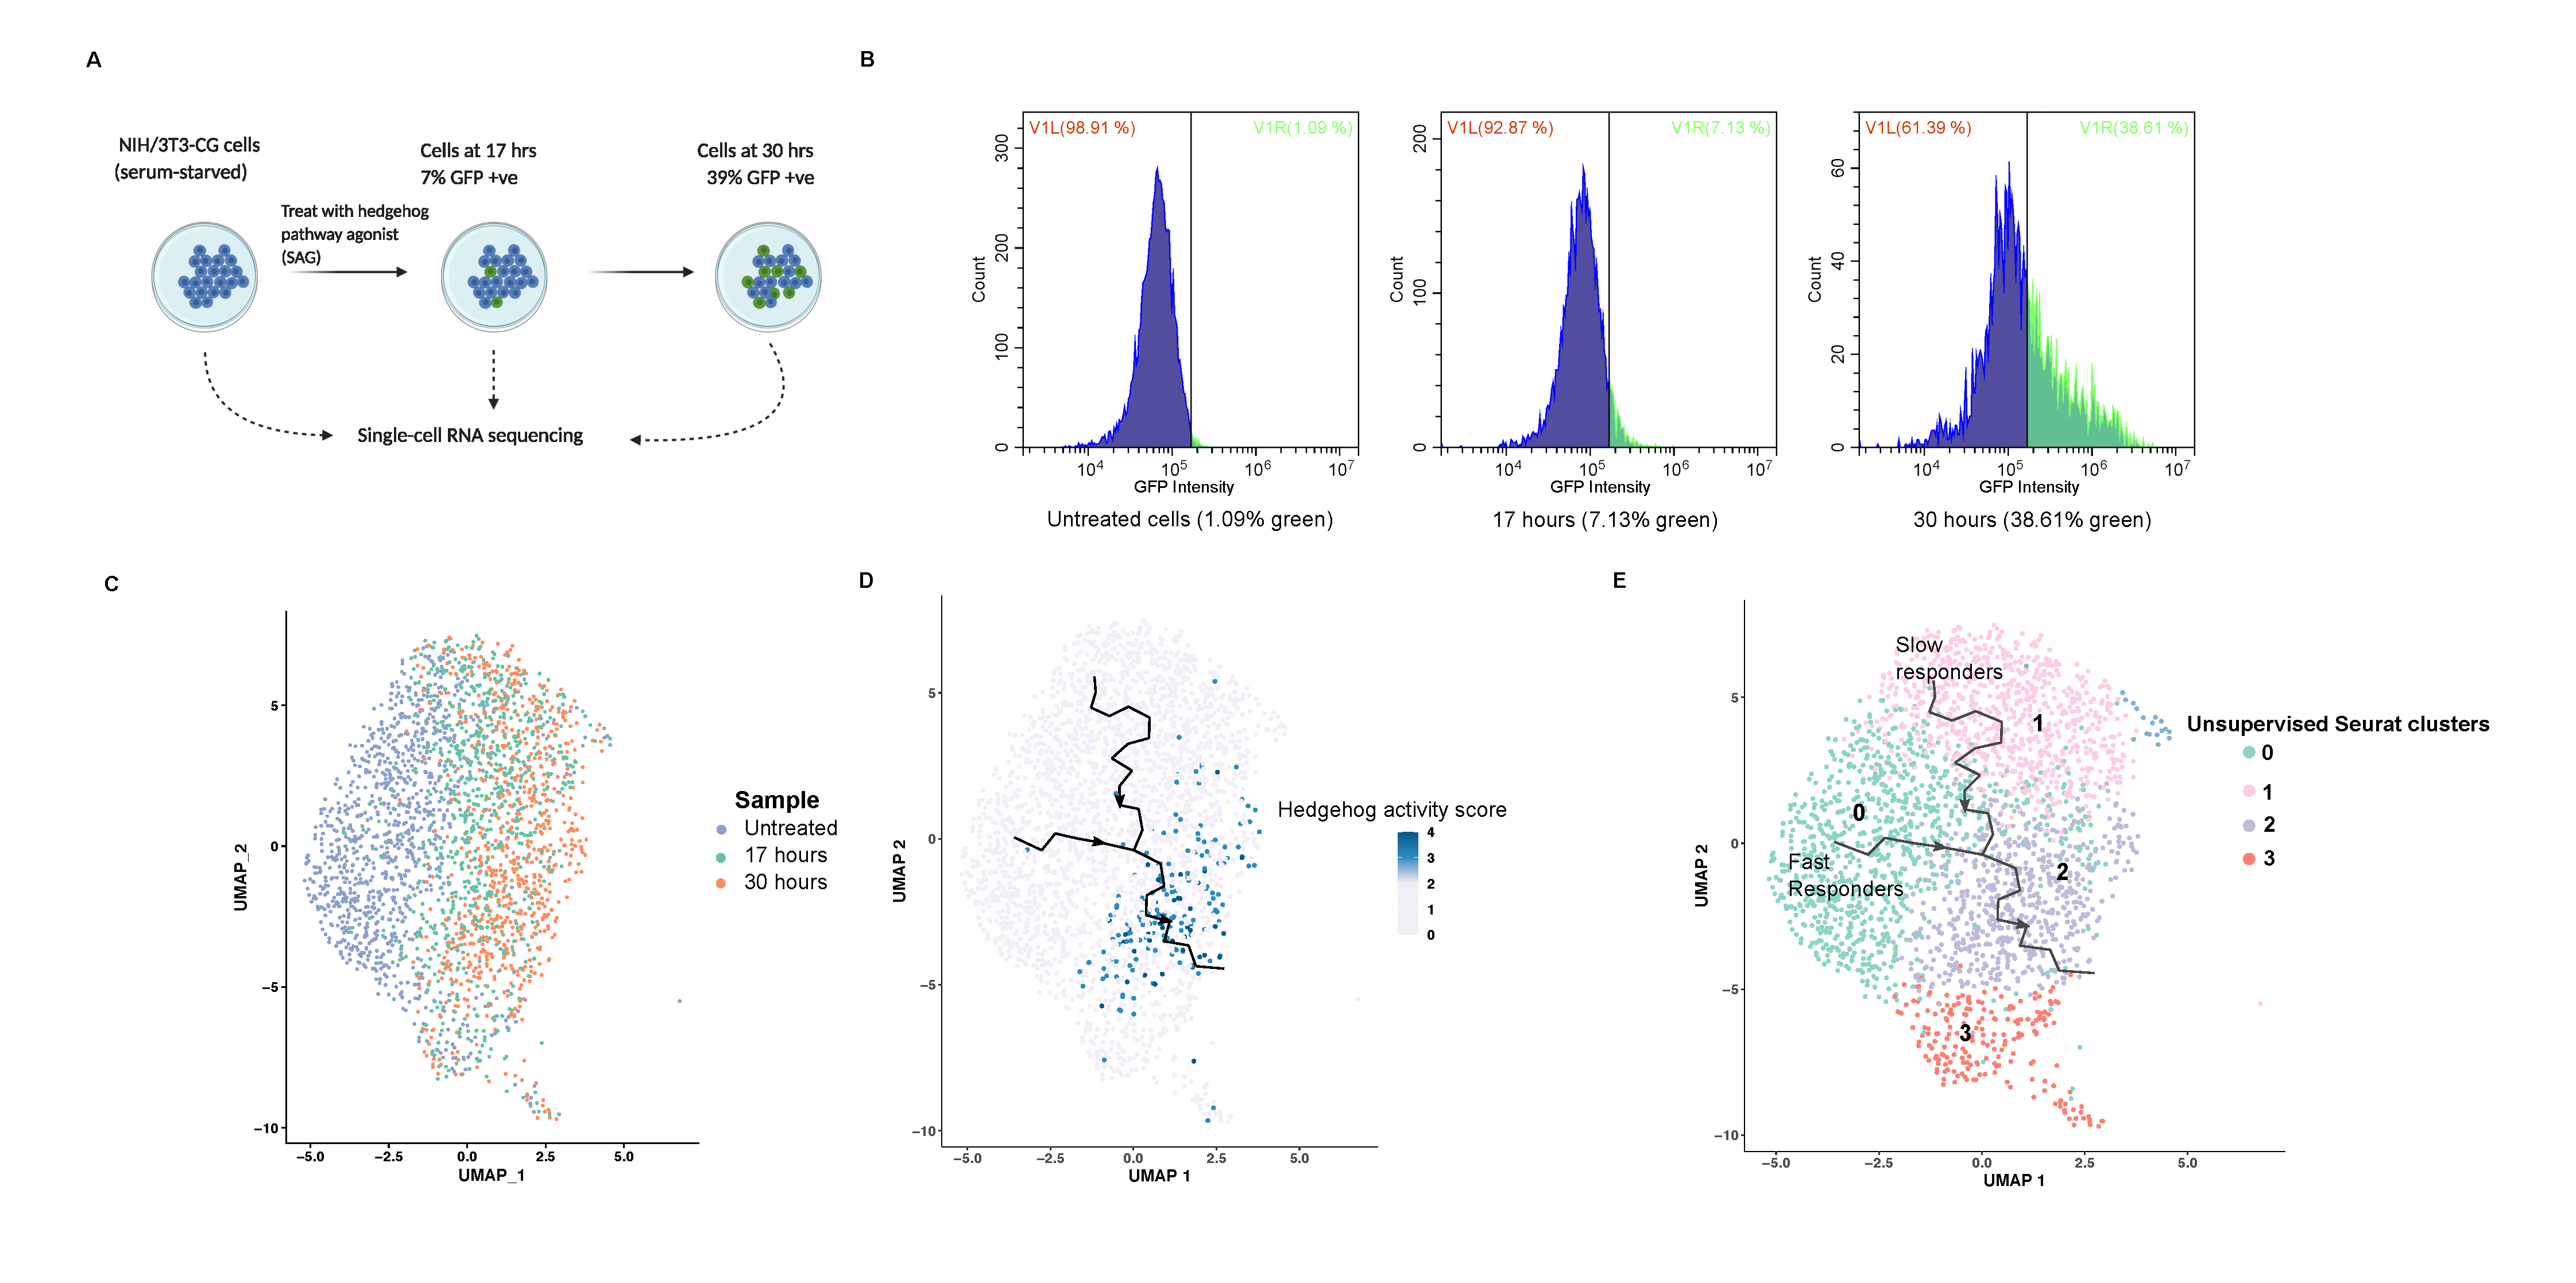
\includegraphics[width=\linewidth]{figures/hedgehog/hh_figure1.pdf}
    \caption[]{%
        \textbf{}
    }
    \label{fig:hh_figure1}
\end{figure}

We first asked whether clonal cells growing in the same environment show variability in their responses to HH signaling. To address this question, we used NIH3T3-CG cells which are an established model of HH signaling \cite{Pusapati2018-gs,Kinnebrew2019-gt}. Treating these cells with SAG activates the pathway, resulting in elevated activity of Gli transcription factors \cite{Briscoe2013-ze,Lee2016-bf,Kong2019-wo}. This increased activity of Gli is read out by a genome-integrated GFP reporter gene regulated by eight Gli binding sites (Supplementary Figure 1). To assess variability in the HH response we treated NIH3T3-CG cells with SAG and monitored the response of the GFP reporter gene by flow cytometry (Figure 1A). Although monocultures of NIH3T3-CG cells are clonal and are grown in the same controlled environment, we detected significant cell-to-cell variability in reporter gene expression in response to SAG (Figure 1B). For example, at 30 hours post SAG treatment only 39\% of cells had activated the reporter gene, whereas by 92 hours most cells responded (Supplementary Figure 2). We observed similar variability of response in multiple experimental replicates grown on different days and derived from multiple single-cell clones (Supplementary Figure 3).  The data support a unimodal distribution using Hartigan’s dip test\cite{Hartigan1985-zq}. What accounts for the difference between fast and slow responding cells in monocultures with no genetic or environmental variation?

\subsection{Fast and slow responding NIH3T3-CG cells}


We asked whether cells that respond quickly to SAG derive from untreated cells with expression profiles that are distinct from the slow responding cells. To do this, we performed scRNA-seq on cells at 0, 17, and 30 hours after the addition of SAG. We chose the 30 hour time-point since we observed close to maximal cell-to-cell variability in response at this time-point and the 17 hour time-point is about halfway in-between the start of the response and 30 hours. The SAG addition was done in a staggered manner to process all three scRNA-seq libraries in a single batch (Methods, Supplementary Figure 4). We first visualized the cells at the three time-points using UMAP (Figure 1C) and performed unsupervised clustering of cells. On the same UMAP plot, we colored the cells for Hedgehog response using four Hedgehog response genes (Methods) and observed a region of the UMAP where the responding cells reside (Figure 1D). We observed similar results when we visualized cells using Principal Components Analysis (PCA) (Supplementary Figure 5), but UMAP highlighted the local differences between cells better and captured all the variation in two dimensions.

Next, we used trajectory analysis \cite{Qiu2017-uz,Trapnell2014-ho} to identify the cell states from which slow and fast responders derive. We observed two distinct trajectories after SAG treatment that lead towards cells expressing genes indicative of the Hedgehog response (Figure 1D). Fast responding cells start in cluster 0 and follow a trajectory that leads into cells that express Hedgehog responsive genes at 17 and 30 hours (Figure 1E). Slow responding cells start in cluster 1 and many of these cells remain in the same cluster at 17 and 30 hours, while other slow responding cells follow a trajectory that leads towards but does not reach Hedgehog responding cells. We interpret this result to mean that untreated NIH3T3-CG cells consist of two distinct subpopulations, one that is primed to respond quickly to SAG (fast-responders - cells in cluster 0 of Figure 1E) and another that takes longer to respond (slow responders - cells in cluster 1 of Figure 1E). Very few untreated cells lie outside these two clusters. The fact that these two subpopulations of untreated cells, identified through unsupervised clustering, are in distinct regions of the UMAP plot suggests that their global mRNA expression profiles define the fast and slow responding states.

We used a second trajectory analysis software, Slingshot \cite{Street2018-ak}, to verify the trajectory inferred using Monocle. Both Monocle and Slingshot were both rated accurate trajectory inference tools in a review evaluating different trajectory analysis software \cite{Saelens2019-fq}. We observed similar results with Slingshot (Supplementary Figure 6) as we did with Monocle; we find two different trajectories, one starting from the fast responders and another from the slow responders, leading to the hedgehog responsive cells.

One hypothesis that might explain cell-to-cell differences in the timing of the Hedgehog response between the two subpopulations would be transient activation of Hedgehog signaling in the absence of ligand. Cells that are in the midst of transiently activating the pathway would then respond faster to extracellular ligand than the remaining cells. To test this hypothesis, we looked for subsets of cells that expressed targets of Hedgehog signaling. In the unstimulated population we did not observe individual cells with activation of Hedgehog target genes (Supplementary Figure 7). Thus, Hedgehog signaling appears to be regulated tightly enough that stochastic activation of the pathway in the absence of ligand is unlikely to account for the cell-to-cell differences in cellular response after the addition of ligand.

\subsection{Differences in cell cycle state do not fully explain fast and slow responding cells}

We next asked whether differences in the cell-cycle state of cells might explain the differences between the fast and slow responding cells. We serum-starve cells prior to hedgehog treatment to synchronize the cells. We used the global expression profiles of serum-starved untreated cells to assign them to different phases of the cell cycle and asked whether fast responding cells were enriched for any specific phase of the cell-cycle. We observed a 1.5 fold enrichment (74.3\% of fast responders vs 50.4\% in the slow responders) of G1 cells in the fast responders compared to the slow responders (Supplementary Figure 8). While we found a statistically significant enrichment, the fact that half of slow responding cells were found in G1 suggests that being in G1 is not sufficient to respond faster. To validate the Seurat cell cycle measurements, we measured the \% of cells in different phases of the cell cycle using Propidium Iodide staining after 24 hours and 48 hours of serum starvation (Supplementary Figure 9A). The computed percent of cells in different phases of the cell cycle after 24 hours of serum starvation agrees with the Seurat estimated cell-cycle fractions. To further test the effect of the length of serum starvation, we serum starved cells to two lengths - 24 hours and 48 hours. We then used Propidium Iodide staining to look at the \% of cells in different phases of the cell cycle. We observe similar amounts of hedgehog response variability after 48 hours of serum starvation as compared to 24 hours of serum starvation (Supplementary Figure 9B) indicating that 24 hour serum starvation is sufficient. We conclude that cell-cycle differences do not fully explain the differences between fast and slow responding cells.
\subsection{Differentially expressed transcription factors and pathways in the fast-responder cells}

We identified genes that are differentially expressed between untreated cells defined as either fast or slow responding (Methods). We focused on the top 300 genes, ranked by fold-change, that were statistically significantly different between the fast and slow populations (Supplementary Data 1). We use these 300 genes in subsequent analyses as markers of the fast responder state. Among the 300 genes, 37 genes are TFs; we decided to focus on the TFs in the differentially expressed genes because we hypothesize that fluctuations in TF activities account for the differences between fast and slow cells. The 37 differentially expressed TFs are shown in Supplementary Table 1. 

We also asked if any biological pathways were among differentially expressed genes between the fast and slow responding cells through a Gene Ontology(GO) analysis (Methods). We observed that the cholesterol biosynthesis pathway is significantly enriched in the set of genes differentially expressed between the two groups (Supplementary Table 2, Enrichment = 28.38, p-value = 1.7e-4, n = 5 out of 13 genes). Cholesterol boosts Hedgehog signaling by serving as a cofactor for Smoothened \cite{Huang2018-iz,Huang2016-er,Kinnebrew2019-gt,Luchetti2016-cd,Radhakrishnan2020-ii}. Increased cholesterol biosynthesis may contribute to the phenotype of fast responding cells. 


\subsection{Slow responding cells pass through the fast state before responding}

Slow responding cells might respond more slowly because they first have to enter the fast responding state from their current state or because they follow a distinct set of cellular states that lead to the Hedgehog response. We distinguished between these two possibilities by examining the set of genes that come on in the slow responders at later time points. Specifically we examined cells from hour 17 and hour 30 in the slow-responding cluster (cluster 1 in Figure 1D) and asked what genes are differentially expressed compared to untreated cells in the same cluster. When the slower responders respond, we observe that they turn on the gene signature of the fast responding cells. At 17 hours these cells express 32 of the 300 fast responder genes (total number of DE genes = 117), and at 30 hours they express 48 of the 300 fast responder genes (total number of DE genes = 196), these are both statistically significant enrichments over random expectation (Hypergeometric test; p-values = 7.9e-27, 1.8e-37). We interpret this result to mean that the slower responders take longer to follow the same trajectory as fast responding cells rather than following a different trajectory.

\subsection{Overexpressing candidate transcription factors partially recreates the fast responder gene signature}

%figure2
\begin{figure}[t!]  
    \centering
    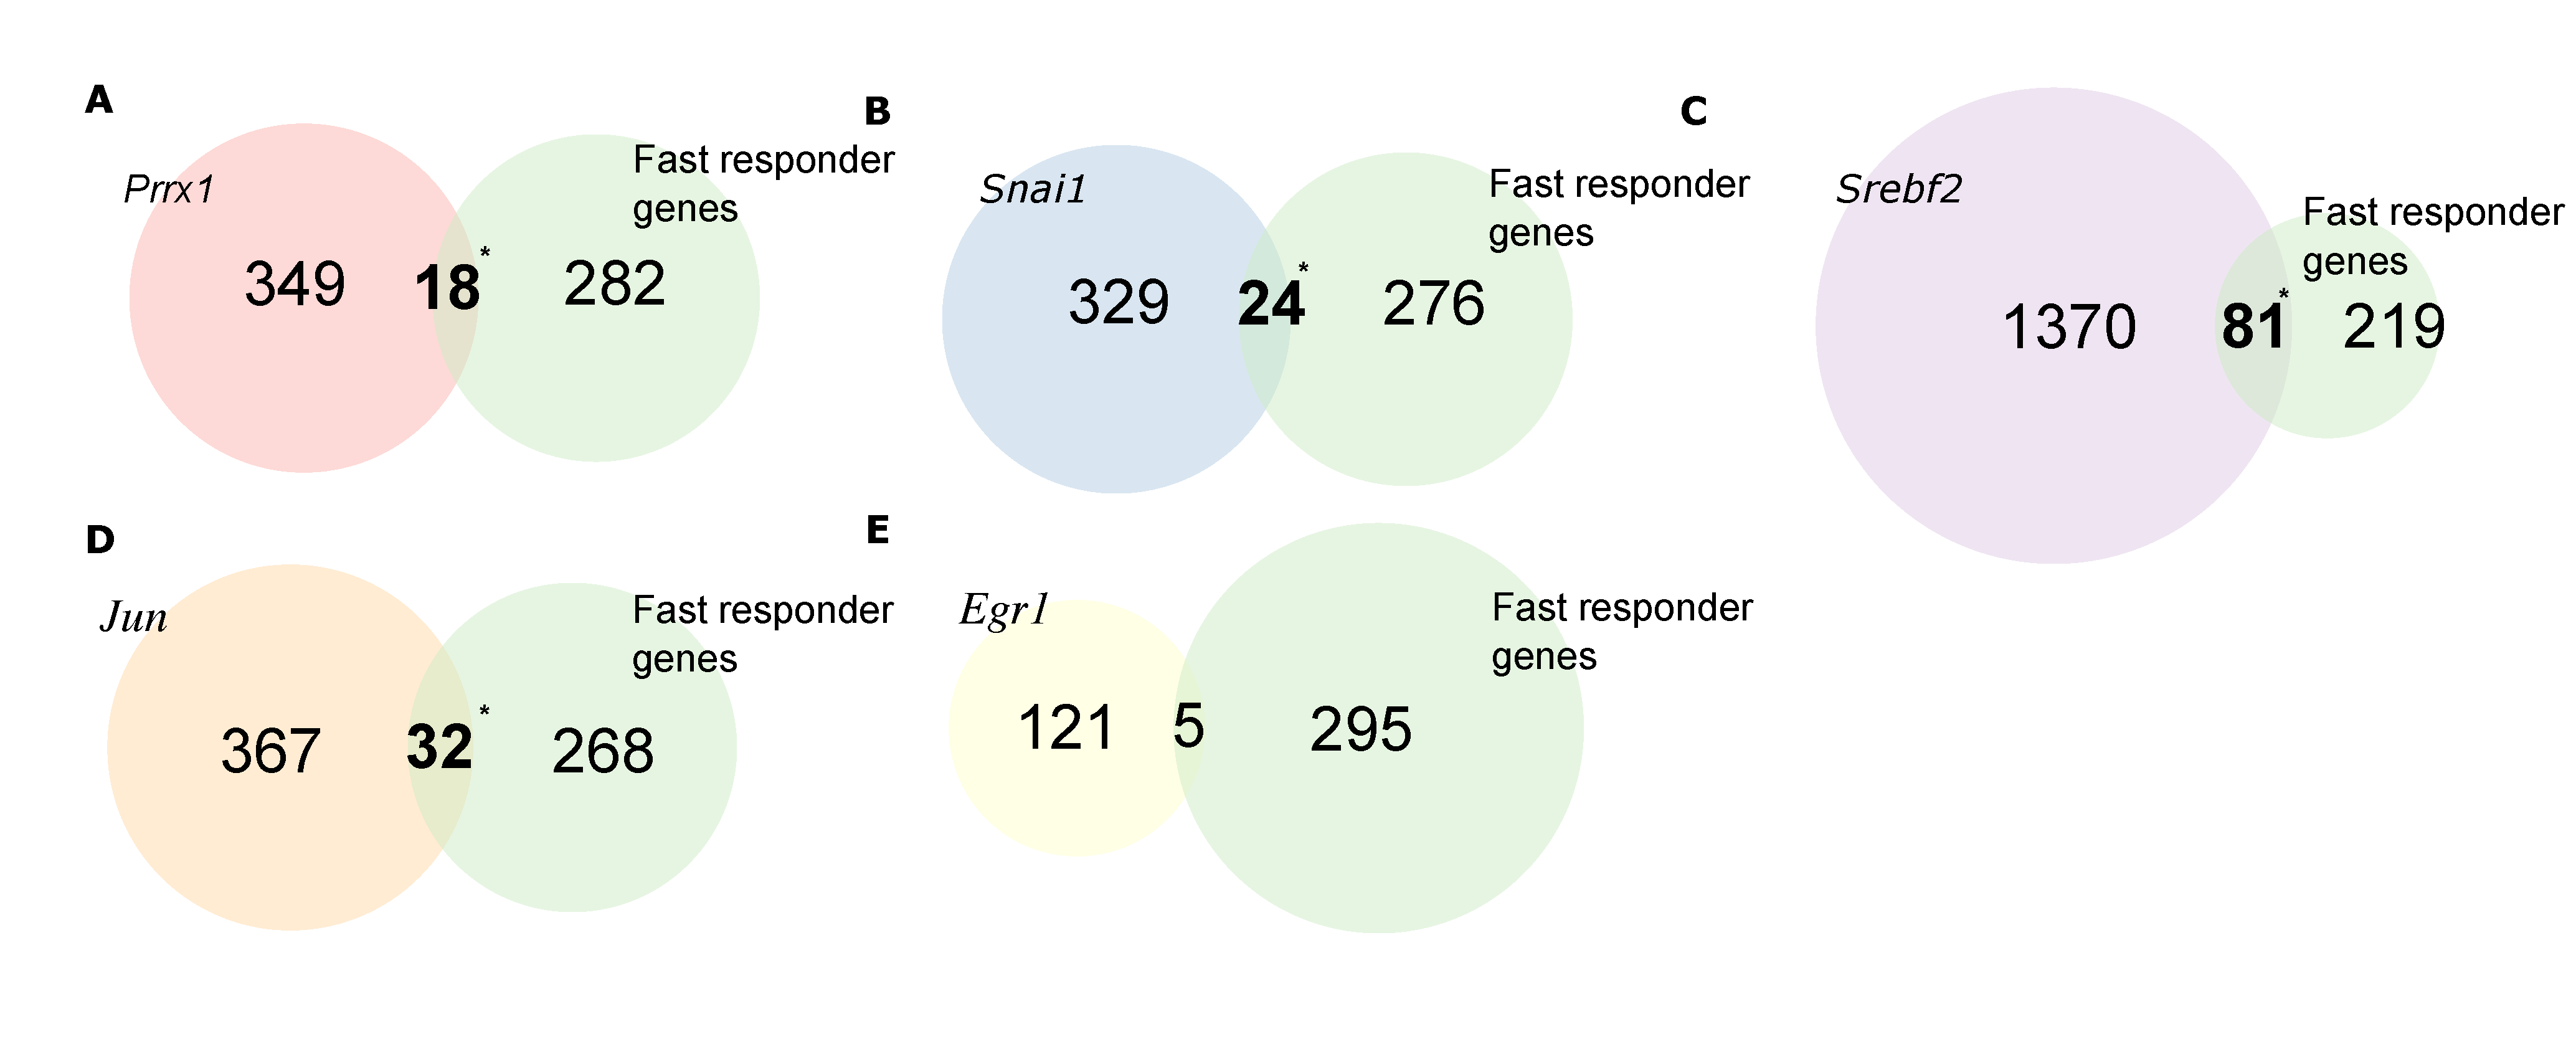
\includegraphics[width=\linewidth]{figures/hedgehog/hh_figure2.pdf}
    \caption[]{%
        \textbf{}
    }
    \label{fig:hh_figure2}
\end{figure}

Our results suggest that fluctuations in the activities of a small set of transcription factors and/or the upregulation of cholesterol biosynthesis pathway causes the differences between fast and slow responding cells. To test this hypothesis, we over-expressed these transcription factors and the cholesterol biosynthesis pathway and measured the bulk expression profiles of the resulting cells. We focused on the top three transcription factors based on fold-change in the fast responder cells (Supplementary Table 1): Jun, Egr1 and Prrx1. We also tested the transcription factor Srebf2, the main regulator of the cholesterol biosynthesis pathway \cite{Horton1998-lj}, because this pathway is upregulated in the fast responder cells (Supplementary Table 2). We chose Snai1 as a control transcription factor due to its lower fold change (fold-change 1.21). The expression of the top differentially expressed transcription factors co-localize with the fast responder cell populations (Supplementary Figure 10). We designed plasmids encoding the coding regions of Jun, Egr1, Prrx1, Srebf2 and Snai1 under the control of a strong CMV promoter, and with an mCherry gene downstream of the TF to measure transfection efficiency (Supplementary Figures 11, 12). Separately, we used a plasmid containing an mCherry reporter gene driven by a CMV promoter as a transfection control plasmid. We transfected these plasmids into NIH3T3-CG cells and performed bulk RNA-seq. We identified genes that are differentially expressed before and after transfection of each of the transcription factors but not after the control transfection (Supplementary Data 2, 3, 4, 5, 6).

Overexpression of four of the five transcription factors (Prrx1, Snai1, Jun and Srebf2) individually misexpressed a significant number of the fast responder genes (Figure 2; Hypergeometric test: p-values = 9.7e-4, 6.3e-7, 1.2e-10, 1.9e-16), whereas Egr1 overexpression did not (p-value = 0.13). We found that overexpressing Snai1, our control TF with a lower fold-change, also misexpressed a significant number of fast-responder genes indicating that even TFs with lower fold-changes might be involved in creating the fast-responder signature in cells. We found that the union of all four of these TFs (Prrx1, Snai1, Jun and Srebf2) resulted in 115 out of the 300 fast responder gene signature, this is smaller than the naive sum of the individual target genes and indicates overlap in the sets of target genes regulated by the TFs. Overall, we interpret this result to mean that each TF independently regulates a subset of the fast-responder signature.

\subsection{Prrx1 is a regulator of the fast responder state}
%figure3
\begin{figure}[t!]  
    \centering
    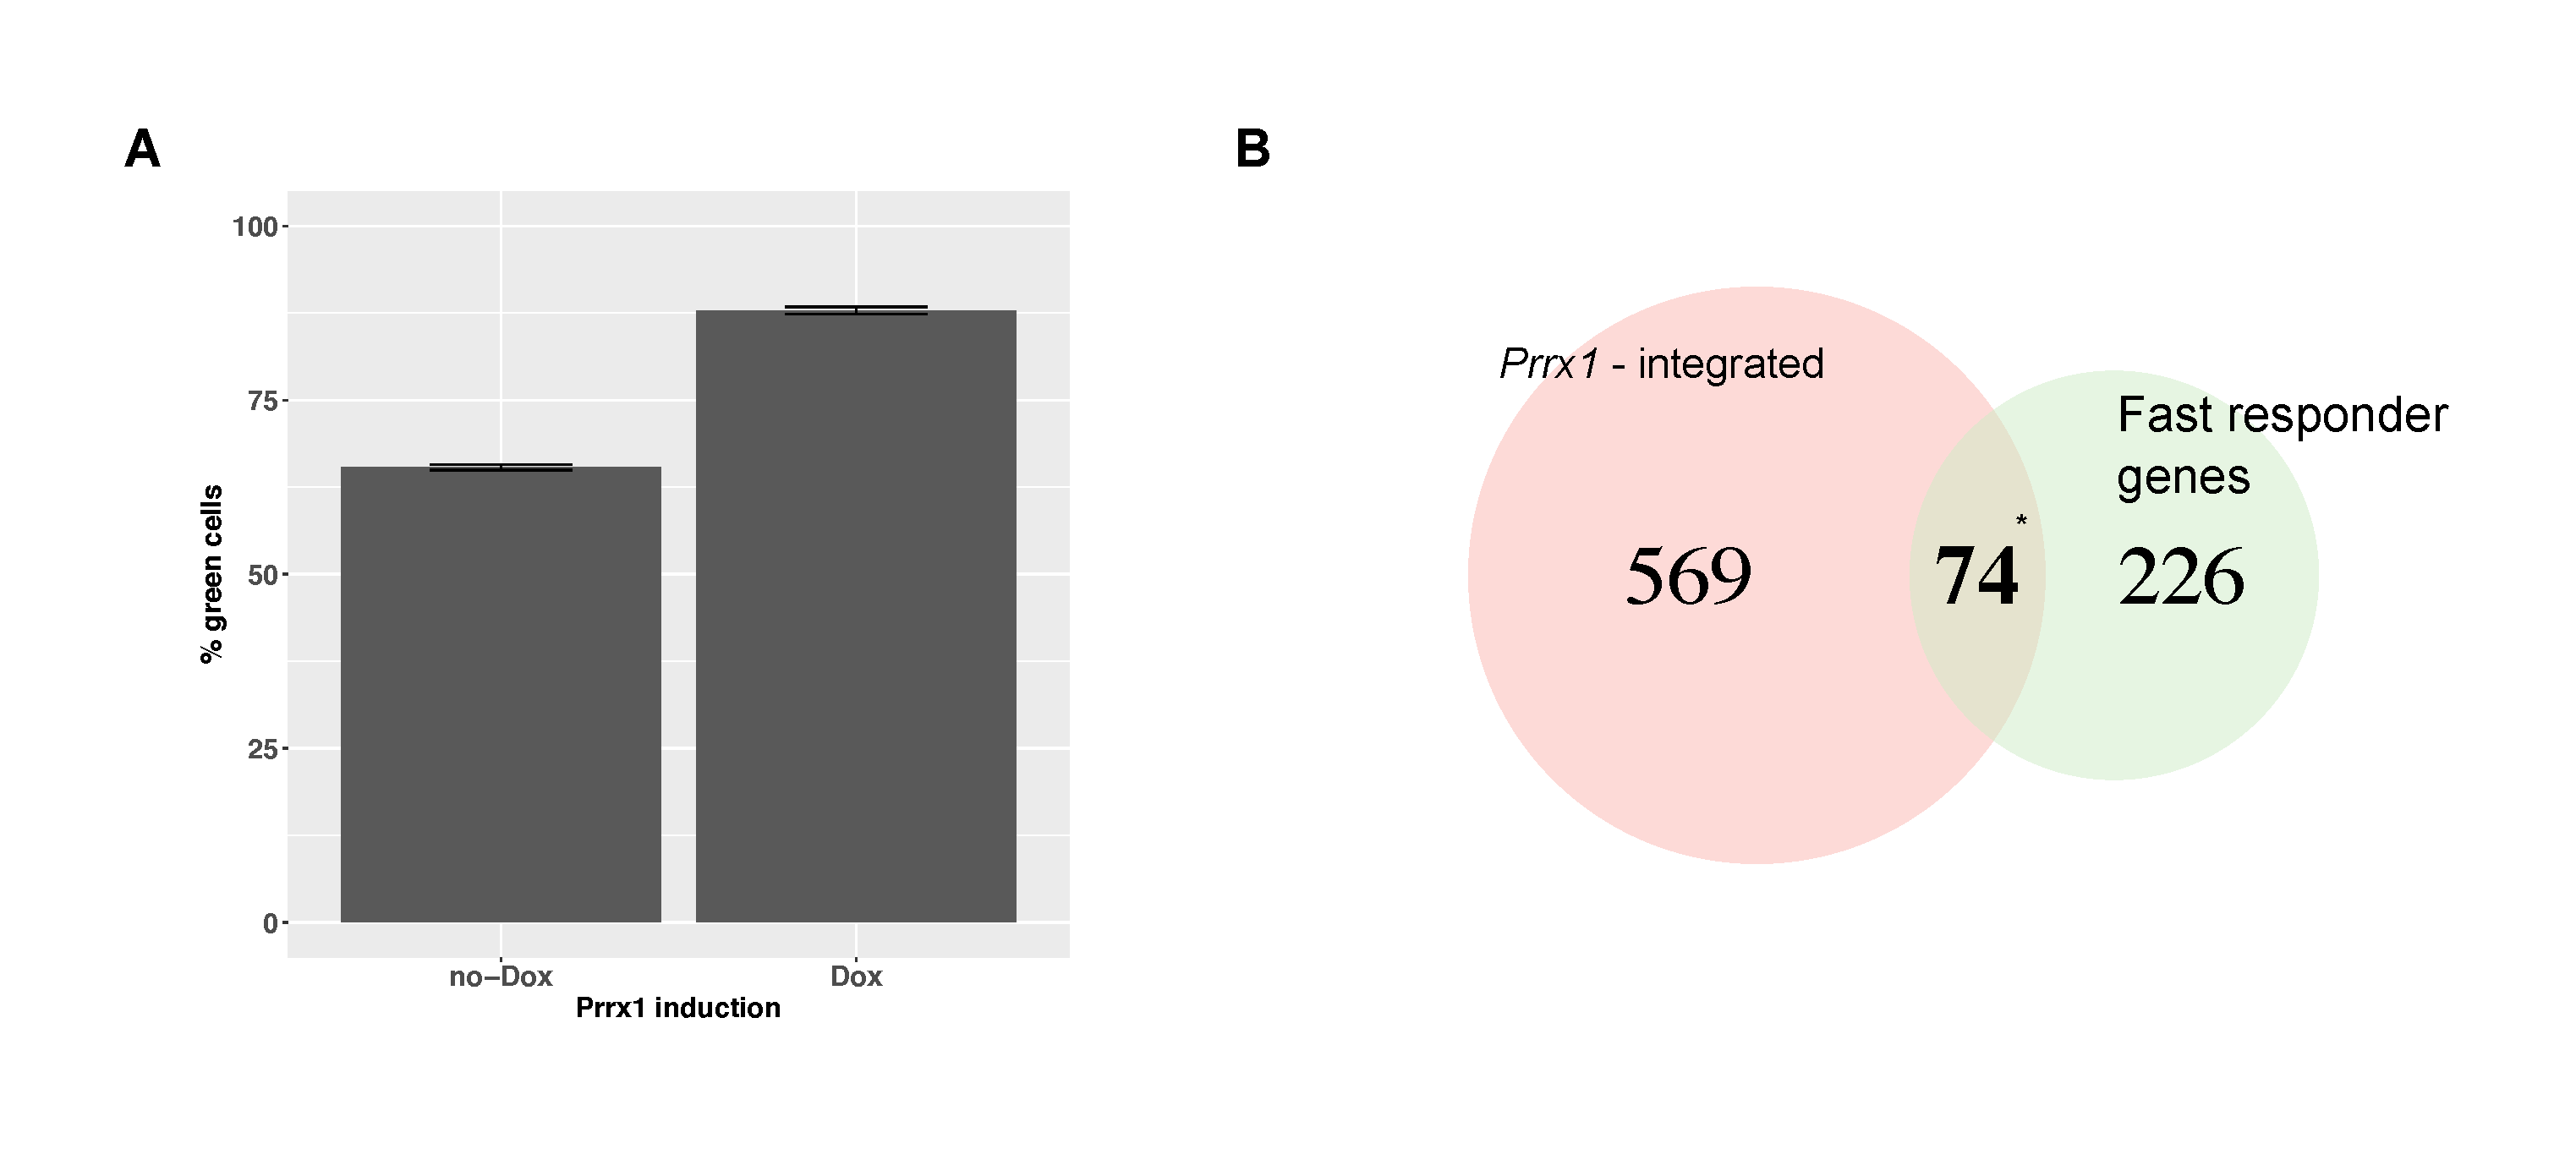
\includegraphics[width=\linewidth]{figures/hedgehog/hh_figure3.pdf}
    \caption[]{%
        \textbf{}
    }
    \label{fig:hh_figure3}
\end{figure}
We next asked whether the overexpression of any of these transcription factors was sufficient to increase the fraction of cells that respond to the Hedgehog signaling pathway. To test this prediction we engineered cells, using lentiviral vectors (Methods, Supplementary Figures 13, 14), carrying Dox-inducible (Supplementary Figure 15) versions of Prrx1, Srebf2 and Snai1 integrated into their genomes. This allowed us to compare the fraction of cells that respond to SAG when a TF is either induced or uninduced. We prioritized the list of transcription factors to test since we could not test all of them. We chose Srebf2 since it is the main regulator of the cholesterol biosynthesis pathway which is the top differentially enriched pathway in the fast responding cells (Supplementary Table 2) and showed a statistically significant enrichment. Additionally, we chose Prrx1 and Snai since they showed strong enrichment for competent genes in the transfection assay and because of their roles as developmental TFs.

Inducing Prrx1 expression resulted in more cells responding to the Hedgehog pathway (Figure 3A, Supplementary Figures 16, 17). In the +Dox condition, at 32 hours post SAG treatment, 87.9\% of cells become GFP+, whereas in the -Dox condition 65.4\% of cells become GFP+. We did not observe a difference between the two groups with the induction of Snai1 (Supplementary Figure 18). Strong induction of Srebf2 was toxic to cells, and at induction levels that were not toxic we did not observe an increase in the response to SAG  (Supplementary Figure 19). From these results, we conclude that Prrx1 plays a role in the regulation of the Hedgehog response.

Bulk RNA-seq profiles from Prrx1 induced cells (Supplementary Data 7) revealed a stronger overlap with fast responding genes than in the plasmid overexpressed cells (Figure 3B; n = 74 out of 300, p-value = 4e-34, enrichment = 5.37 fold). This stronger measured response is likely because in transiently transfected cells only a subset of the cells are expressing Prrx1 whereas in the lentiviral transduced cells all the cells in the population are overexpressing Prrx1. Induction of Prrx1 results in significant enrichment of genes involved in the cholesterol biosynthesis pathway (adjusted p-value = 0.025, enrichment = 10.42, n = 4 out of 13 genes in the pathway). Prrx1 induction also results in the upregulation of Gli2, the primary effector TF of Hedgehog signaling \cite{Kong2019-wo,Briscoe2013-ze,Lee2016-bf}. Gli2 is regulated post-translationally by Hedgehog signaling, so the upregulation of Gli2 in uninduced cells may result in a larger pool of Gli2 protein to activate when the pathway is activated. We observe slight leaky expression in the transduced clone with a fold change of 1.5 X which could underlie some of the higher response in the -Dox condition compared to wild-type cells in Figure 1. A previous study used genome-wide CRISPR knockouts \cite{Pusapati2018-gs} to identify regulators of hedgehog signaling and did not find Prrx1 necessary for Hedgehog signaling. Our results indicate that overexpression of Prrx1 can recreate a substantial part of responder signature, which we interpret as the reason more of these cells respond to Hedgehog signaling.

\subsection{Most cells activate the fast responder gene signature upon Prrx1 induction}
%figure4
\begin{figure}[t!]  
    \centering
    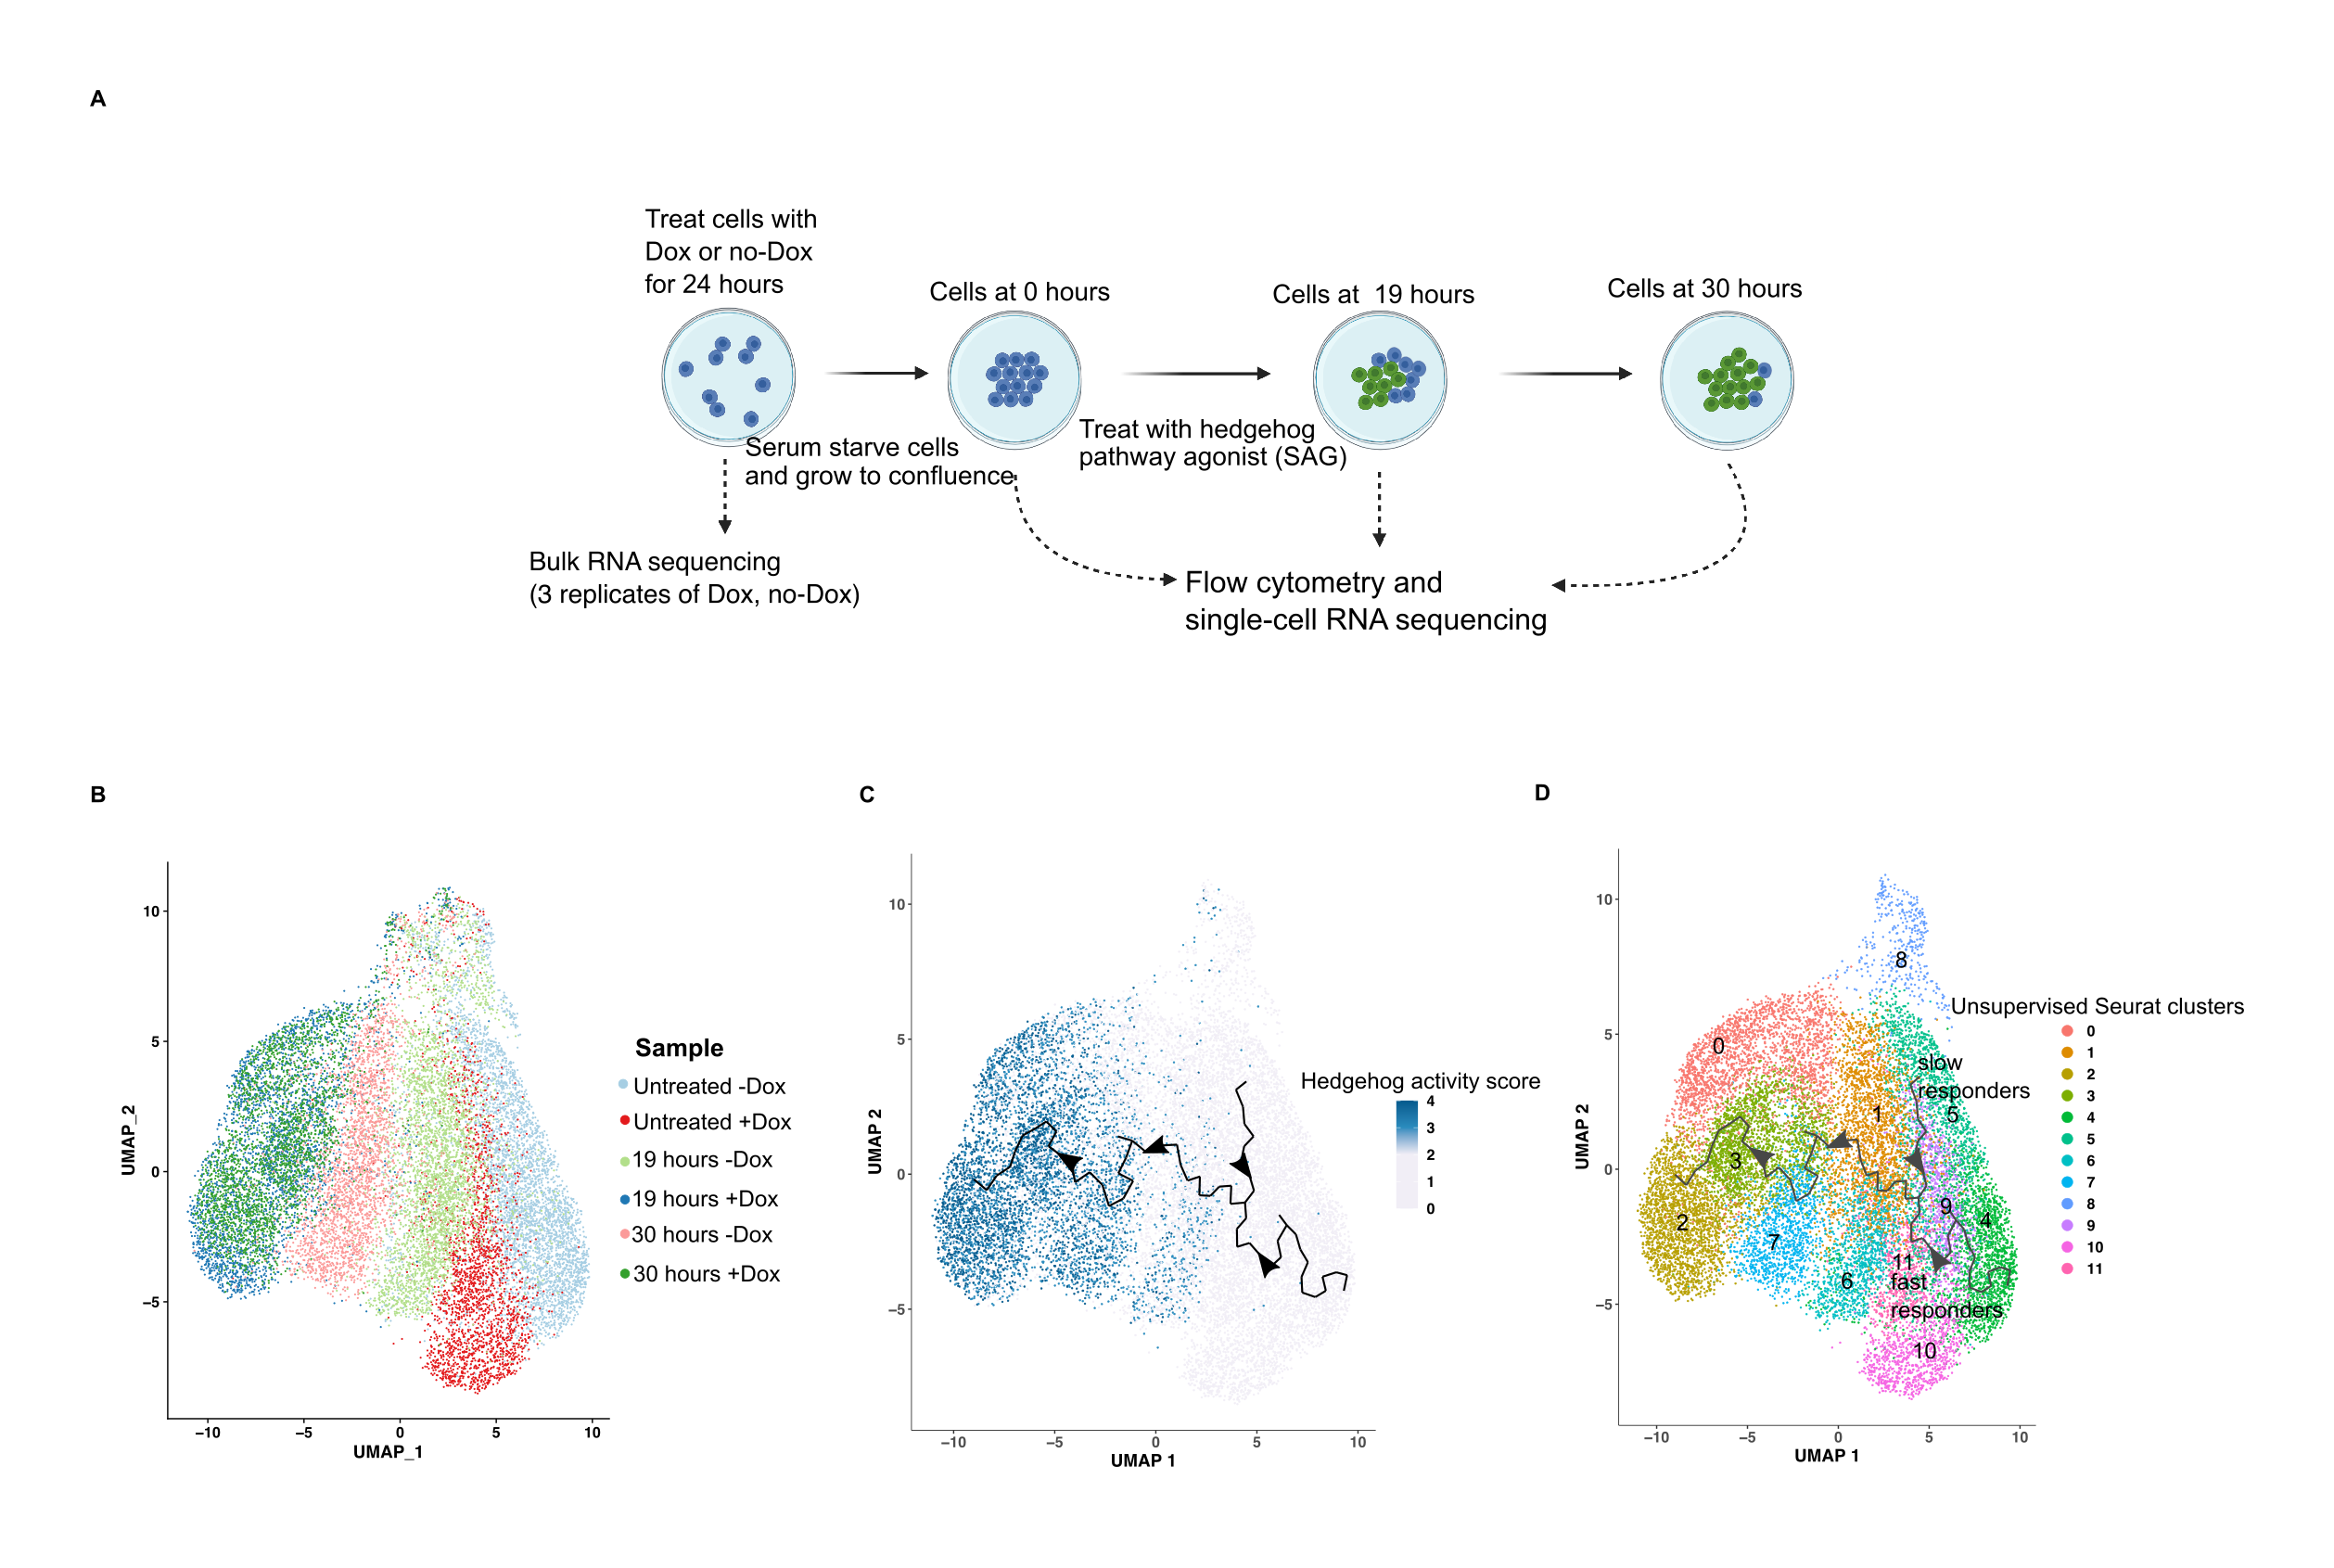
\includegraphics[width=\linewidth]{figures/hedgehog/hh_figure4.png}
    \caption[]{%
        \textbf{}
    }
    \label{fig:hh_figure4}
\end{figure}
We next examined the trajectory taken by cells overexpressing Prrx1. We generated scRNA-seq profiles of Prrx1-induced and uninduced cells followed by stimulation with SAG (Figure 4A). We started with the cells carrying the genome-integrated inducible Prrx1 cassette described in the previous section. We grew cells in the absence or presence of Dox, to induce Prrx1 expression, and measured the HH response by flow cytometry. We again observed a larger response in Prrx1-induced cells than in uninduced cells (Supplementary Figure 20). We then collected cells at three time points after SAG treatment for both Prrx1-induced and uninduced cells and performed scRNA-seq.

Prrx1 induced cells follow a faster and stronger response trajectory compared to their uninduced counterparts. When Prrx1 is not induced, cells from each time-point again cluster separately, suggesting a steady progression of response to SAG through time (Figure 4B). By contrast, when we induced Prrx1 expression with Dox, cells at the 19 hr and 30 hr time point cluster together, suggesting a faster response to SAG induction (Figure 4B). Overlaying the Hedgehog response on these clusters supports this interpretation as Prrx1-induced cells at 19 hours show similar levels of the Hedgehog response as induced cells at 30 hrs (Figure 4C). However, even at 30 hrs induced and uninduced cells do not cluster together, which suggests that Prrx1 induction results in a stronger response to Hedgehog in cells that do respond. Taken together, these results show that the induction of Prrx1 causes more cells to respond to SAG, and that those cells that do respond, respond faster and stronger than cells that do not express Prrx1.

The trajectory analysis also revealed differences between induced and uninduced cells in the early response to SAG that are consistent with the idea that Prrx1 causes cells to adopt fast-responding expression profiles. Uninduced cells again showed distinct converging trajectories from slow and fast responding states (clusters 4, 5 in Figure 4D), but Prrx1-induced cells respond primarily along the fast trajectory. In addition, the Prrx1-induced cells start from a position along the fast trajectory that is closer to the later time points than the uninduced cells (clusters 9, 10, 11 in Figure 4D), which suggests that they are “further along” the fast trajectory than uninduced cells even before stimulation with SAG. 

We next asked whether inducing Prrx1 creates more fast-responding cells. To detect fast responding cells in this experiment we used a model-based cell-type classifier Garnett \cite{Pliner2019-vn}. We trained the classifier to learn the features of fast-responding and slow responding cells using the cells from the untreated condition shown in Figure 1. We then used the classifier to classify untreated cells grown in the +Dox and -Dox conditions as fast responders and slow responders. In the untreated cells grown in -Dox condition, the classifier classified 19\% of cells as fast-responders, 48\% as slow responders and 33\% of the cells as unknown. The fast responders in this group separate from the slow responders in the UMAP plots and are slightly ahead in the response trajectory even before SAG treatment  (Supplementary Figure 21 A, B). In contrast, in the untreated cells from the +Dox condition the classifier classified 91\% of cells as fast-responders, 2\% slow-responders and 7\% as unknown (Supplementary Figure 21 C, D). Thus in the presence of Dox, the majority of cells display the fast-responder expression signature. We infer from this result that inducing Prrx1 generates a fast responder cell-state which makes more cells respond to the Hedgehog agonist, as early as 19 hours.

\section{Discussion}

We hypothesized that fluctuations in the activities of TFs produce transient changes in gene expression that can generate phenotypic differences among clonal cells in the same environment. Consistent with this hypothesis, we showed that distinct gene expression profiles define fast and slow responding states among clonal NIH3T3-CG cells, and that the activities of a small number of TFs accounts for a substantial fraction of the expression differences that define the two states. The idea that these expression profiles cause differences in the response to Hedgehog signaling is supported by the observation that overexpression of Prrx1 is sufficient to generate part of the fast responding expression signature and drive a faster and stronger response to Hedgehog in a larger fraction of cells. However, because Prrx1 only accounts for part of the fast responding expression signature, there must be fluctuations in other TFs\cite{Sigal2006-ds}, or other types of signaling molecules, that generate the fast responding cell state. Much deeper sequencing of unstimulated cells might reveal groups of differentially expressed target genes that could indicate which TFs and signaling molecules are involved, much the same way in which coherent differential expression of the cholesterol biosynthesis pathway suggested the involvement of Srebf2 in the fast responding state. Alternatively, if the transient activation of non-TFs (e.g. receptors, kinases)\cite{Colman-Lerner2005-ln} underlies the fast responding state, then it will be necessary to identify specific changes in gene expression that are diagnostic of changes in the activities of such genes.

We observe parallels between our model underlying variability in the Hedgehog response and other previously described systems where fluctuations of a few key molecules underlie cell-to-cell variability in phenotypic outcomes. For example, differences in the levels of a few apoptotic regulator proteins prior to drug treatment determines how fast cells die in the presence of an apoptosis inducing ligand \cite{Spencer2009-hh}.  Fluctuations of a few resistance genes in cancer cells results in cell states that are resistant to cancer drugs, \cite{Emert2021-ej,Shaffer2020-ff} though the exact mechanisms underlying the emergence of such cell states remains unknown and is hypothesized to involve the fluctuation of multiple upstream transcription factors. In stem cells, fluctuations of a key transcription factor Nanog affect whether cells differentiate or remain in the pluripotent state \cite{Miyanari2012-zv,Torres-Padilla2014-mz}. A recent study using fluorescence microscopy determined that most of the variability in the JAK-STAT signaling response can be attributed to fluctuations in the molecular content of cells \cite{Topolewski2022-bw}. Differences in the amount of transcription factors between cells have been hypothesized to underlie disease due to haploinsufficiency where some cells in a population are unable to express the transcription factor above a required threshold.\cite{Cook1998-es,Kemkemer2002-iw} Single-cell transcriptomic approaches, such as those used in this study, can shed light on the specific molecular differences between cells that result in heterogeneity of response.

Our study also has important implications for improving the efficiency of cellular assays. For example, reprogramming assays can be made more efficient if we understand why some cells are successfully reprogrammed while other cells result in ‘dead-end’ states \cite{Biddy2018-ct,Graf2009-qr,Francesconi2019-ol}. Fluctuations of transcription factors in cells prior to reprogramming might underlie the heterogenous outcome. For example, in hematopoietic progenitor cells, levels of a stem cell marker determine  which lineage a cell differentiates towards \cite{Chang2008-kv}. Isolating cells with different levels of such proteins may improve reprogramming efficiency. Identification of TFs, like Prrx1 in this study, that dampen noise of a system could also aid in the design of synthetic circuits where noise is a significant obstacle \cite{Murphy2010-zb}.

We have inferred the Hedgehog response trajectories using computational methods that look at gene expression similarities between single-cells. A complementary measurement of the trajectory would involve using transcribing molecular barcodes to tag the cells prior to single-cell RNA sequencing \cite{Kong2020-ox}. This approach could reveal how fast cells transition between the slow and fast responder states \cite{Hormoz2016-wo,Stumpf2017-ne,Larsson2021-ub}. We have used overexpression experiments to infer the role of Prrx1 in the fast response. Using GFP fused versions of Prrx1 would help separate the fast responder population from the slow responders and perform functional assays on these subsets of cells. Finally, we have used a widely used cell-culture model of Hedgehog signaling, and how our findings apply to in vivo Hedgehog signaling remains to be tested. 

One future direction of this work will be to determine whether the fast responding state is specific for Hedgehog signaling or if this state makes cells differentially responsive to other signaling pathways and perturbations. We speculate that similar variability in the activities of different TFs may underlie other phenotypic differences among genetically identical cells and experimental approaches similar to ours can be used to uncover this variability.

\section{Materials and Methods}

\subsection{Cell Culture}
We grew NIH/3T3-CG cells and their derivatives in DMEM media supplemented with sodium pyruvate, 10\% Bovine Serum (Gibco 16170078) and 1\% Penicillin-Streptomycin. We grew the cells in an incubator maintained at 37 degrees celsius with 5\% CO2.

\subsection{RNA Sequencing Experiments}
We generated single-cell RNA sequencing libraries using the 10X Single Cell 3’ Reagent Kits v3.1 (10X genomics 1000269). We first released the cells from the cell culture flasks by adding Trypsin 0.25\%. We then prepared a cell suspension by following manufacturer’s instructions and targeting a final capture of 2000 cells for every sample. We then proceeded with library construction as described in the 10X protocol. We sequenced the final libraries at the DSIL and MGI at Washington University in St. Louis. Bulk RNA sequencing was performed using the services of Novogene corporation. Briefly, we extracted total RNA from cells, performed initial QC and shipped it to Novogene where library preparation and sequencing were performed targeting 20 million reads per sample. 

\subsection{RNA sequencing analysis}
We obtained counts for each transcript in each cell by using Cell Ranger version 3.1.0 (https://support.10xgenomics.com/single-cell-gene-expression/software/pipelines/latest/using/count).  We analyzed the cell by count matrix using the standard analysis workflow of Seurat version 3.1.5.\cite{Butler2018-jc,Stuart2019-ra} For quality control, we kept cells that had at-least 10,000 UMIs per cell, had < 20\% of UMIs mapped to mitochondrial genes, and had between 2000 and 8000 genes covered. After QC, for the initial single-cell sequencing experiment we were left with transcriptome measurements for 1,192 cells for the untreated time-point, 797 cells at 17 hours and 899 cells at 30 hours. For the second single-cell RNA-sequencing experiment using the inducible Prrx1 cell-line, under the no-Dox condition we were left with 4532 cells at the untreated time-point, 3726 cells at 19 hours and 2645 cells at 30 hours after QC. Under the Dox condition, after QC we were left with 2362 cells at the untreated time-point, 3014 cells at 19 hours and 2645 cells at 30 hours. 

We performed dimension reduction of single cells using UMAP\cite{McInnes2018-sm}. We identified differentially expressed genes between clusters using the FindMarkers function in Seurat.  We identified pathways that were enriched in the set of differentially expressed genes using the Gene Ontology web resource\cite{Ashburner2000-id,Mi2019-pi,Gene_Ontology_Consortium2021-mx}.

We performed trajectory analysis using Monocle3 version 1.0.0\cite{Trapnell2014-ho,Qiu2017-uz} and Slingshot version 1.4.0 \cite{Street2018-ak}. The Monocle workflow consists of a series of steps. The first step involves pre-processing of the data and dimensionality reduction. We started with the cell by gene matrix that was pre-processed using Seurat and the UMAP dimension reduction results for trajectory analysis. We next identified clusters of the cells using the cluster\_cells method of Monocle. We then used the learn\_graph method to learn a trajectory graph and ordered the cells according to pseudotime using the order\_cells method. We were able to infer directionality on the Monocle trajectory using the timepoint information that the cells come from (each timepoint is a different library on the 10X platform), the arrows in Figure 1 go from the earlier time-point to later-time-points as the cells progress through the SAG treatment. For trajectory inference using Slingshot, we used the same cell by gene matrix pre-procesed using Seurat, UMAP dimension reduction results and passed it to the slingshot method. We did not specify the start and end clusters for either Monocle or Slingshot.  More details regarding the parameters used for the various programs are available in the R notebooks made available in the Zenodo repository listed below. 

We computed the hedgehog pathway activity score for each cell by looking at the mRNA expression of four genes - the GFP reporter,  Gli1, Gli2 and Ptch1. For each of the four genes in each cell, we assigned a score of 1 if the gene is detected above background expression level and 0 if not. We then sum over all four genes to obtain a score in the range 0-4 for each cell.

For bulk RNA-sequencing analysis we pseudo-aligned the reads to the mouse reference cDNA using Kallisto version 0.43.0 \cite{Bray2016-hc}. We used the counts from Kallisto to identify differentially expressed genes using DESEQ2 version 1.26.0 \cite{Love2014-lk}. We used a false-discovery rate of 0.05 to annotate genes as differentially expressed across conditions.

\subsection{Enrichment Calculation}
We performed enrichment analysis of the genes that are perturbed when a TF is overexpressed using a hypergeometric test. We detect ~14,000 genes in our single-cell data, out of which there are 300 genes in the fast-responder gene signature. Using a hypergeometric test, for each TF overexpression experiment we ask if the overlap of the 300 genes with the number of genes that change expression upon TF overexpression is a statistically significant enrichment under the null hypothesis of no enrichment. We indicate statistically significant enrichments in the figures with an asterix. We used the hypergeom function in the scipy.stats Python package to compute the enrichment p-values.

\subsection{Hedgehog Assay}
We performed the Hedgehog assay on NIH/3T3-CG cells as previously reported in Pusapati et. al. Briefly, we grew cells to confluence in media containing regular amounts (10\%) of serum. We then switched the cells to low serum media (0.5\% serum) overnight, and treated the cells with the Hedgehog pathway agonist SAG (Tocris Biosciences Part number: 4366) at 100 nM concentration. We measured the amount of fluorescence in the cells on a flow cytometer after allowing for the appropriate time period of response depending on the experiment. For the initial experiment in Figure 1 we collected cells at 17 hours and 30 hours. For the Prrx1 overexpression single-cell experiment we collected cells at 19 hours and 30 hours. For both these experiments, we treated cells that didn’t receive SAG as untreated cells or time-point zero. The time course treatments were done in a staggered manner so that all the cells could be harvested at the same time for single-cell RNA sequencing library preparation. This enabled us to process all the cells in one batch to minimize experimental variability for single-cell RNA sequencing. 

\subsection{Flow Cytometry}
We performed the flow cytometry experiments on a Beckman Coulter Cytoflex S instrument. We performed QC based on manufacturer provided QC beads prior to every experiment. We used the same cytometer gain settings for all experiments. To prepare cells for flow cytometry, we first released cells from culture wells by adding Trypsin and then added appropriate volume of culture media to neutralize Trypsin. We gated cells based on forward scatter and side scatter and measured GFP intensity on the FITC channel. We used a negative control sample (no SAG added) to identify the cutoff for the GFP intensity and measured the proportion of responders as the percentage of cells above this cutoff under different experimental conditions.

\subsection{Plasmid Transfection}
To transfect the plasmids overexpressing the transcription factors we used Lipofectamine 3000 (Invitrogen L3000001) reagent. We used 2.5 ug of DNA per transfection reaction, on a six-well plate, and followed manufacturers instructions for amounts of Lipofectamine and P3000 reagents. We measured transfection efficiency on a flow cytometer using the fluorescence of a reporter gene on the transfected plasmid or a control plasmid transfected in parallel. If we observed sufficient transfection efficiency (> 50\% of cells express transfected plasmid) we extracted total RNA, 24 hours post transfection, from the cells and performed bulk RNA sequencing. The control plasmid used is a mCherry reporter gene driven by a CMV promoter.

\subsection{Lentiviral generation and transduction}
We chose the canonical coding transcripts and sequences for all the genes from UniProt \cite{noauthor_2021-be}. We then cloned the protein coding regions of Prrx1, Snai1 and Srebf2 to the pINDUCER21 Dox-inducible lentiviral vector \cite{Meerbrey2011-ew} using the services of Genscript (Addgene 46948, Supplementary Figures 6 and 7). We used the pINDUCER21 system since it allows us to control the level of over-expression of a gene with precision by adding different levels of Doxycycline to the cell growth media. This construct also has a fluorophore (miRFP670) on it which allows us to isolate cells that contain the integrated construct. The Hope Center at Washington University in St. Louis generated high-titer lentiviruses using the constructs. Detailed lentivirus generation protocol used by the Center is described in their publication \cite{Li2012-if}.

We used the generated virus to transduce the NIH3T3-CG cells and used 4 ug/ml polybrene to maximize transduction efficiency. After 24 hours of cell-growth in the transduction media, we replaced the media with fresh regular media. We used a fluorescent marker of integration to sort single-cells (miRFP670) using a Sony SH800 cell-sorter and grew out single-cell clones that we evaluated for TF induction. 

We evaluated single-cell clones based on induction levels assessed by qPCR. For induction of clones we used Doxycycline (Dox) at a concentration of 500 ng/ml. For transcription factor induction followed by RNA-seq experiments, cells were treated with Dox for a period of 24 hours to induce TF expression. We identified one clone for each transcription factor that offered a good level of inducibility (Supplementary Figure 8). We then used these clonal cell lines as a model to study the effect of TF overexpression on the Hedgehog assay. 

To perform the Hedgehog assay, we grew the cells in two different growth conditions - in one condition we added Dox to the media and in the other condition we omitted Dox. We then grew the cells to confluence, for 24 hours, and added SAG to both populations of cells to initiate the Hedgehog pathway response. We used flow cytometry to determine the effect of the overexpression of these transcription factors on the response to Hedgehog stimulation by measuring the GFP fluorescence of the reporter gene on the FITC channel. 

\subsection{qPCR Run and Analysis}
We first extracted total RNA from cells using the Qiagen RNEasy kit(Qiagen 74004). We generated cDNA from the total RNA using the RDRT reagent (Sigma RDRT-100RXN) by following manufacturer's protocol. We then mixed SYBR green PCR master mix(Applied Biosystems 4301955) with 2 ul of cDNA from the previous step, water and primers to set up a standard qPCR run on the QuantStudio instrument (Applied Biosystems). For the transcription factor induction experiments using the transduced cell-lines, we used the no-Dox sample as the baseline for computing the delta Ct value. We used HPRT primers to normalize as a within sample control for TF expression (Supplementary Table 3). We analyzed the results of the QuantStudio run using the Design and Analysis 2 software from Thermo Fisher.

\section{Data Availability}
The raw single-cell and bulk RNA sequencing data from this publication are available from GEO under the accession numbers GSE203134 and GSE206154. Analysis notebooks used for the analysis of single-cell data are available for download at Zenodo: https://doi.org/10.5281/zenodo.6981764

\clearpage
\section{Supplementary Figures}

\clearpage
\section{Supplementary Tables}

\begin{supptable}[p]
\centering
\caption{List of top transcription factors overexpressed differentially expressed in the fast responders compared to the slow responders}
\begin{tabular}{ cccc }
\toprule
\textbf{Transcription Factor} & \textbf{Fold-change (fast responders vs slow responders)} & \textbf{Adjusted p-value} \\
\midrule
Jun & 1.54414 & 3.66E-23 \\
Egr1 & 1.41021 & 3.08E-33 \\
Prrx1 & 1.39419 & 1.56E-50 \\
Srsf5 & 1.33099 & 1.53E-45 \\
Maged1 & 1.28932 & 4.09E-36 \\
Asap1 & 1.27863 & 1.15E-25 \\
Fos & 1.26675 & 1.20E-11 \\
Jund & 1.24454 & 2.63E-21 \\
Sub1 & 1.2398 & 1.73E-32 \\
Aebp1 & 1.2163 & 3.99E-16 \\
Tsc22d1 & 1.21429 & 6.90E-15 \\
Nr2f2 & 1.21215 & 1.43E-18 \\
Snai1 & 1.21021 & 4.09E-19 \\
Cebpd & 1.20596 & 0.00216788 \\
Foxg1 & 1.19574 & 1.56E-19 \\
Cited2 & 1.1919 & 8.05E-14 \\
Hlf & 1.19155 & 1.22E-26 \\
Lbh & 1.19117 & 3.12E-20 \\
Ebf1 & 1.18643 & 1.64E-09 \\
Atf5 & 1.18342 & 1.95E-11 \\
Zfp36l1 & 1.17283 & 1.73E-07 \\
Fosb & 1.1675 & 2.45E-12 \\
Nfib & 1.16638 & 1.11E-17 \\
Nfix & 1.16262 & 1.66E-18 \\
Hnrnpd & 1.1563 & 2.40E-17 \\
Drap1 & 1.1537 & 5.51E-19 \\
Sap30 & 0.869089 & 2.41E-11 \\
Nr1d1 & 0.868365 & 1.60E-18 \\
Sqstm1 & 0.865831 & 1.34E-07 \\
Ybx1 & 0.862252 & 3.57E-25 \\
Rnps1 & 0.858557 & 2.88E-17 \\
Tgif1 & 0.848734 & 6.74E-18 \\
Klf9 & 0.819257 & 2.41E-17 \\
Atf4 & 0.817134 & 7.62E-23 \\
Ptma & 0.809741 & 3.20E-33 \\
Tmpo & 0.793335 & 7.15E-26 \\
Ddit3 & 0.533202 & 8.25E-58 \\
\bottomrule
\end{tabular}
\label{tab:hedgehog_tableS1}
\end{supptable}

\begin{supptable}[p]
\centering
\caption{List of signaling pathways enriched in the fast responder cells compared to slow responders}
\begin{tabular}{ p{3cm}p{3cm}p{3cm} }
\toprule
\textbf{Pathway} & \textbf{Genes in fast responder gene signature and in the pathway (Total number of genes in pathway)} & \textbf{Enrichment over random expectation (FDR adjusted p-value)} \\
\midrule
Cholesterol biosynthesis & 5 (13) & 28.38 (1.7e-4) \\
Integrin signaling pathway & 20 (189) & 7.81 (6.2e-10) \\
Ubiquitin proteasome pathway & 5 (65) & 5.68 (4.1e-2) \\
Cytoskeletal regulation by Rho GTPase & 6 (79) & 5.60 (2.3e-2) \\
\bottomrule
\end{tabular}
\label{tab:hedgehog_tableS2}
\end{supptable}


\begin{supptable}[p!]
\centering
\caption{Primer sequences used for qPCR}
\begin{tabular}{ cc }
\toprule
\textbf{Primer} & \textbf{Sequence} \\
\midrule
Prrx1-fwd & GCAGGACAATGACCAGTTGAAC \\
Prrx1-rev & CGTGCGAGATCTTCTCGAAC \\
Snai1-fwd & CGTGTGTGGAGTTCACCTTCC \\
Snai1-rev & GTACCAGGAGAGAGTCCCAGAT \\
Srebf2-fwd & GGACATCGACGAGATGCTACAG \\
Srebf2-rev & TCTGTGGCTCCACCATTGTT \\
Hprt-fwd & CTGGTGAAAAGGACCTCTCGAAG \\
Hprt-rev & CCAGTTTCACTAATGACACAAACG \\
\bottomrule
\end{tabular}
\label{tab:hedgehog_tableS3}
\end{supptable}